\chapter{序論}
\label{chap:introduction}

本章では本研究の背景、それを踏まえた上での研究の目的、そして文書の構成について述べる。

\section{本研究の動機}
 昨今ではVirtual Realityが開発が進んでいる\cite{vrtrendShiny}。Virtual Realityはコンピューターによりシュミレーションされた拡張現実がユーザの動きにインタラクティブに反応することをいう。図\ref{trends}は年代別に制作されたVirtual Realityの数を示している\cite{vrtrendSamuel}。\\

\begin{figure}[htbp]
\begin{center}
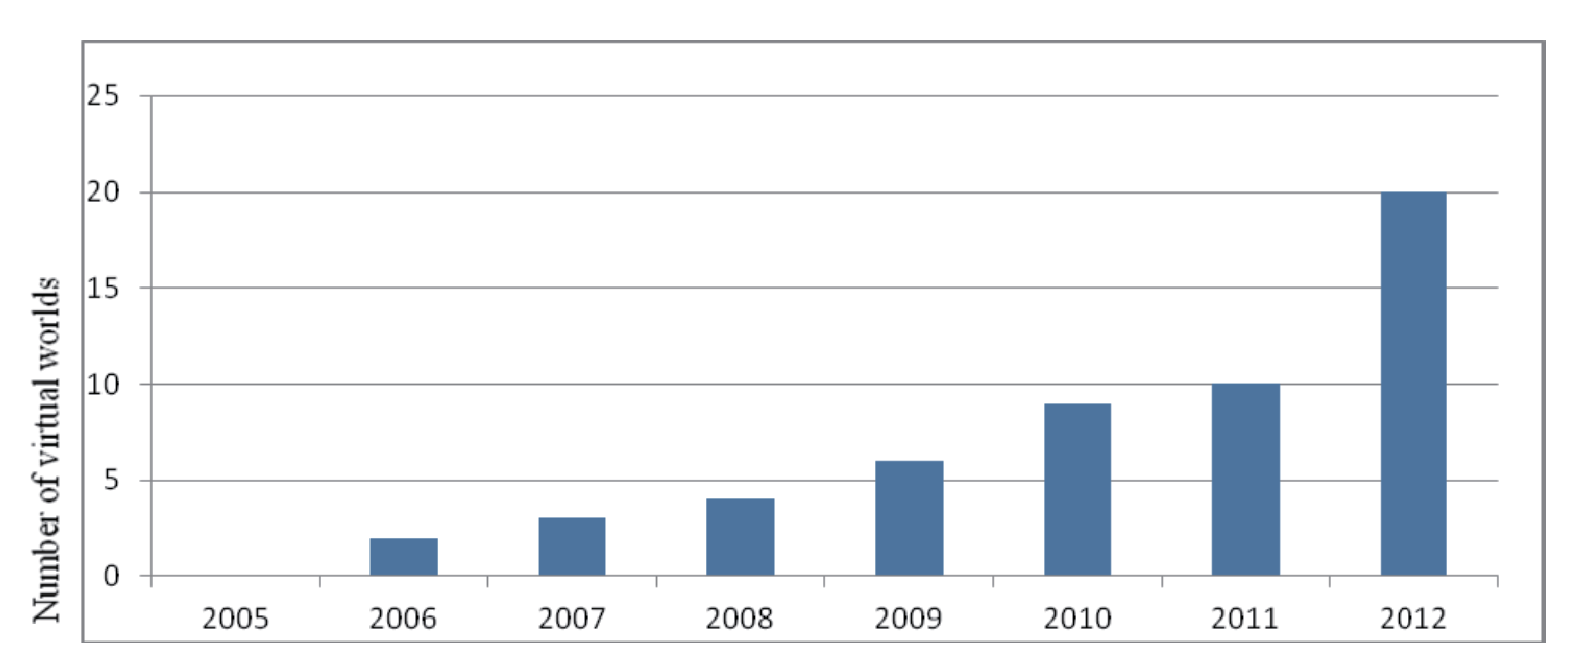
\includegraphics[width=15cm]{eps/vrTrends.eps}
\caption{Virtual Reality トレンド}
\label{trends}
\end{center}
\end{figure}

 現実世界を越えた体験をしたいというニーズに応えるために、企業や研究団体が開発を進めている。人々の欲求の中には物理的壁を越えて遠くにいる人と会いたい、時間的壁を越えて過去に旅行をした時の思い出を再び体験したい、自ら好きな映画の登場人物となって刺激を感じてみたいなどというものが含まれる。Virtual Realityは拡張現実をより現実的に感じさせるために、映像の見せ方、インタラクションの行われ方、音の聞こえ方を正確に実現しなければならないため開発に労力と時間がかかる\cite{vrtrendShiny}。\\
 しかし実は毎晩睡眠中に人々は拡張現実を体験しているのだ。辞書 『大辞泉 第二版』によると、夢とは「睡眠中にあたかも現実の経験であるかのように感じる一連の観念や心像のこと」\cite{dream}と書かれている。中でも明晰夢は1867 年に Saint Denys により研究が行われて以来\cite{saintDenys}、心理学者や哲学者の間で研究が進められてきた。明晰夢とは睡眠中にみる夢のうち、自分で夢であると自覚しながら見ている夢のことである。経験者は夢の状況を自分の思い通りに変化させられる、言い換えれば拡張現実を体験することができると語られてきた。スタンフォード大学博士の Stephen LaBergeは1987 年に The Lucidity Institute を設立し、明晰夢を見るためのステッ プを Mnemonic Induction of Lucid Dreams (The MILD Technique) で紹介した\cite{LaBerge}。しかしThe MILD Techniqueを習得するには特殊な訓練が必要となり、労力が必要で誰もが気軽に始められるものとは言い難い。そこで誰もが比較的簡単に明晰夢をみるとで、拡張現実を体験できるツールの開発が望ましい。

\section{本研究の目的}
 本研究ではVirtual Realityに変わって明晰夢に着目する。そして寝る前にスマートフォンのアプリを起動するだけで睡眠中に拡張現実を体験できる、MemoryDreamの提案と試作をする。具体的にはユーザーの思い出に関連した音声や画像が持つ明晰夢の誘発可能性について証明する。誰もが簡単に夢を操作できる方法を見つけることができれば、物理的に会うことのできない人と会話をしたり、授業で学んだ内容を復習したり、過去の思い出でもう一度過ごすことで睡眠をより楽しむことができるなど、これまでにない新しい睡眠のスタイルの実現となる。\\
 人生の1/3を過ごす睡眠時間をより有効的に使うことができれば人類の発展に大いに繋がる可能性が高い。睡眠の質の向上を目的として、モニタリング機能を備えたデバイスはiSleep\cite{iSleep}やbeddit\cite{beddit}などこれまでに多くの研究が行われてきた。しかし明晰夢を促進するための研究はまだ少ない。タカラトミーが開発した夢見工房\cite{takaratomi}やDreamON\cite{dreamOn}をはじめとする各種スマートフォンアプリが提案されているが、どれも商業目的のものが多く、信頼性の高い実験データを公開していないため有効性については大いに疑問が残る。そこでMemoryDreamは多数の開発者が実現しようとしたことに挑戦し、詳細な実験結果を残したい。

\section{本文書の構成}
第\ref{chap:introduction}章では、本論文を書くに至った動機とその構成を説明している。第\ref{chap:webapi}章では研究背景をユーザーの拡張現実や明晰夢における認識度や要求について事前調査・分析をし、それに基づいてMemoryDreamの開発に反映した点について述べる。第\ref{chap:search}章では睡眠観測や明晰夢促進という目線での先行研究や開発事例を述べたのちに、複数の 観点からMemoryDreamとの比較を行い新しい解決方法について提起する。第\ref{chap:visualize}章ではMemoryDreamがiOSアプリで睡眠中に音を流すという形に至った背景を述べる。第\ref{chap:coding}章では本研究で試作した MemoryDreamについて、その概要、利用方法、システムの概要、実装手法について述べる。第\ref{chap:ledoxea}章では実験方法と、目的に対するMemoryDreamの有効性について試用実験から評価 する。第\ref{chap:result}章では本研究の総括を行い、また今後の展望について議論する。最後に備考を述べる。
